% Documentation for Youpi
% GPL

\documentclass[twoside,a4paper]{article}
\pagestyle{headings}

\usepackage{fullpage}
\usepackage[dvips]{graphicx}
\usepackage{listings}
\usepackage{ecltree}
\usepackage{epic}
\usepackage{rotating}
% \usepackage{draftcopy}

% Constants
\def \codasyl {{\sc CODASYL\ }}
\def \mcd {{\sc MCD\ }}
\def \mld {{\sc MLD\ }}

\begin{document}

\title{{\sc Youpi}'s Merise Analysis}
\author{M. Monnerville\\G. S\'emah\\E. Bertin}

\maketitle

\begin{abstract}
Merise analysis.
\end{abstract}

% \tableofcontents
\listoftables
\listoffigures
\newpage

\section{Data Dictionnaries}

% ----------------------------- IMAGE -----------------------------------------------
\subsection{Data Dictionnary of {\tt Image} entity}
\begin{sidewaystable}[!h]
\centering
\footnotesize{
\begin{tabular}{|l|l|l|c|c|l|}
\hline
Full name & DB field name & Description & Unit & Type & Display Format\\
\hline
Sky footprint & {\tt skyfootprint} & Footprint of image on sky & deg & Multi-polygon & {\tt \%8f}\\
Image name & {\tt name} & Image name (without the {\tt .fits} extansion) & - & string & {\tt \%s}\\
Image path & {\tt path} & Path of image file (cluster or local) & - & string & {\tt \%s}\\
Right ascension & {\tt alpha} & Right ascension of field centre & deg & double & {\tt \%02d:\%02d:\%05.2f}\\
Declination & {\tt delta} & Declination of field centre & deg & double & {\tt \%+02d:\%02d:\%04.1f}\\
Equinox & {\tt equinox} & Equinox at time of observation & yr & double & {\tt \%7.2f}\\
Object name & {\tt object} & Object identifiant & - & string & {\tt \%s}\\
Observation date & {\tt dateobs} & Date and time at start of observation & - & datetime & {\it date \%c format}\\
Exposure time & {\tt exptime} & Effective exposure time & s & double & {\tt \%9.2f}\\
Magnitude zero-point & {\tt photc} & Magnitude Zero-point for 1s exposure & mag & float & {\tt \%+8.4f}\\
Extinction coefficient & {\tt photk} & Extinction coefficient at airmass 1 & mag & float & {\tt \%7.4f}\\
Airmass & {\tt airmass} & Airmass at start of observation & - & float & {\tt \%8.4f}\\
Absorption & {\tt absorption} & Absorption at start of observation & mag & float & {\tt \%+7.4f}\\
Checksum & {\tt checksum} & Image file checksum & - & unsigned long long & {\tt \%0x}\\
Gain & {\tt gain} & Detector conversion factor & e-/ADU & vector of floats & {\tt \%8.2f}\\
Ingestion date & {\tt ingestion\_date} & Date and time at start of ingestion & - & datetime & {\it date \%c format}\\
Flatfield & {\tt flat} & Flatfield filename & - & string & {\tt \%s}\\
Mask & {\tt mask} & Mask filename & - & string & {\tt \%s}\\
Ds9 region file & {\tt reg} & Ds9 region filename & - & string & {\tt \%s}\\
Validation flag & {\tt QSOstatus} & Image validation status & - & unsigned char & {\tt \%c}\\
\hline
\end{tabular}}
\caption{Data dictionnary of {\tt Image} entity}
\end{sidewaystable}

% ----------------------------- FITSIN PLUGIN -----------------------------------------------
\subsection{Data Dictionnary of {\tt FITSin plugin} entity}
\begin{sidewaystable}[!h]
\centering
\footnotesize{
\begin{tabular}{|l|l|l|c|c|l|}
\hline
Full name & DB field name & Description & Unit & Type & Display Format\\
\hline
RA offset & {\tt astoffra} & Offset wrt astrometric reference catalogue in RA & arcsec (")& float & {\tt \%8.3g}\\
Dec offset & {\tt astoffde} & Offset wrt astrometric reference catalogue in Dec & arcsec (") & float & {\tt \%8.3g}\\
& {\tt astromaccuracy} & & & &\\
RA std dev & {\tt aststdevra} & Dispersion wrt astrometric reference catalogue in RA & arcsec(") & float & {\tt \%8.3g}\\
Dec std dev & {\tt aststdevde} & Dispersion wrt astrometric reference catalogue in Dec & arcsec(") & float & {\tt \%8.3g}\\
Minimum PSF FWHM & {\tt psffwhmmin} & Minimum Full-Width at Half-Maximum of the PSF & arcsec(") & float & {\tt \%8.3g}\\
Average PSF FWHM & {\tt psffwhm} & Central/average Full-Width at Half-Maximum of the PSF & arcsec(") & float & {\tt \%8.3g}\\
Maximum PSF FWHM & {\tt psffwhmmax} & Maximum Full-Width at Half-Maximum of the PSF & arcsec(") & float & {\tt \%8.3g}\\
Minimum PSF half-light diameter & {\tt psfhldmin} & Minimum half-light diameter of the PSF & arcsec(") & float & {\tt \%8.3g}\\
Average PSF half-light diameter & {\tt psfhldm} & Average half-light diameter of the PSF & arcsec(") & float & {\tt \%8.3g}\\
Maximum PSF half-light diameter & {\tt psfhldmax} & Maximum half-light diameter of the PSF & arcsec(") & float & {\tt \%8.3g}\\
Minimum PSF elongation & {\tt psfelmin} & Minimum elongation of the PSF & - & float & {\tt \%5.2f}\\
Average PSF elongation & {\tt psfel} & Central/average elongation of the PSF & - & float & {\tt \%5.2f}\\
Maximum PSF elongation & {\tt psfelmax} & Maximum elongation of the PSF & - & float & {\tt \%5.2f}\\
Minimum PSF chi2/d.o.f. & {\tt psfchi2min} & Minimum chi2/d.o.f. of the PSF fit & - & float & {\tt \%7.2g}\\
Average PSF chi2/d.o.f. & {\tt psfchi2} & Central/average chi2/d.o.f. of the PSF fit & - & float & {\tt \%7.2g}\\
Maximum PSF chi2/d.o.f. & {\tt psfchi2max} & Maximum chi2/d.o.f. of the PSF fit & - & float & {\tt \%7.2g}\\
Minimum PSF residuals & {\tt psfresimin} & Minimum residuals from the PSF fit & - & float & {\tt \%7.2g}\\
Average PSF residuals & {\tt psfresi} & Central/average residuals from the PSF fit & - & float & {\tt \%7.2g}\\
Maximum PSF residuals & {\tt psfresimax} & Maximum residuals from the PSF fit & - & float & {\tt \%7.2g}\\
Minimum PSF asymmetry & {\tt psfasymmin} & Minimum asymmetry from the PSF fit & - & float & {\tt \%7.2g}\\
Average PSF asymmetry & {\tt psfasym} & Central/average asymmetry from the PSF fit & - & float & {\tt \%7.2g}\\
Maximum PSF asymmetry & {\tt psfasymmax} & Maximum asymmetry from the PSF fit & - & float & {\tt \%7.2g}\\
Minimum number of PSF stars & {\tt nstarsmin} & Minimum number of point-sources per detector used for PSF modeling & - & long int & {\tt \%d}\\
Average number of PSF stars & {\tt nstars} & Average number of point-sources per detector used for PSF modeling & - & long int & {\tt \%d}\\
Maximum number of PSF stars & {\tt nstarsmax} & Maximum number of point-sources per detector used for PSF modeling & - & long int & {\tt \%d}\\
Median background & {\tt bkg} & Median background level & ADU & float & {\tt \%9.4g}\\
Background RMS & {\tt bkgstdev} & Dispersion RMS of the background level & ADU & float & {\tt \%8.3g}\\
Saturation level & {\tt satlev} & Detector saturation level & ADU & float & {\tt \%9.4g}\\
Path to mask & {\tt mask} & Absolute path to mask data & - & string & {\tt \%s}\\
Path to flat & {\tt flat} & Absolute path to flat data & - & string & {\tt \%s}\\
Path to region & {\tt reg} & Absolute path to region data & - & string & {\tt \%s}\\
QualityFITS configuration & {\tt qfconfig} & QF configuration file serialized content (base64 encoding over zlib compression) & - & string & {\tt \%s}\\
HTTP url & {\tt www} & URL to QF output HTML data & - & string & {\tt \%s}\\
Results ingestion log & {\tt qflog} & Results ingestion log & - & string & {\tt \%s}\\
Previous quality evaluation & {\tt prevrelgrade} & Previous QualityFITS-in grading & - & string & {\tt \%s}\\
Previous quality comment & {\tt prevrelcomment} & Previous QualityFITS-in comment & - & string & {\tt \%s}\\
\hline
\end{tabular}}
\caption{Data dictionnary of {\tt FITSin plugin} entity}
\end{sidewaystable}

% ----------------------------- SCAMP PLUGIN -----------------------------------------------
\subsection{Data Dictionnary of {\tt Scamp plugin} entity}
\begin{sidewaystable}[!h]
\centering
\footnotesize{
\begin{tabular}{|l|l|l|c|c|l|}
\hline
Full name & DB field name & Description & Unit & Type & Display Format\\
\hline
Results ingestion log & {\tt log} & Results ingestion log & - & string & {\tt \%s}\\
Scamp configuration & {\tt config} & Scamp configuration file serialized content (base64 encoding over zlib compression) & - & string & {\tt \%s}\\
HTTP url & {\tt www} & URL to Scamp output data & - & string & {\tt \%s}\\
LDAC Files & {\tt ldac\_files} & List of LDAC files used during processing (serialized data) & - & list & {\tt \%s}\\
Thumbnails & {\tt thumbnails} & True if thumbnails of output images (only group \#1) have been created during processing (with convert utility) & - & boolean & {\tt \%s}\\
\hline
\end{tabular}}
\caption{Data dictionnary of {\tt Scamp plugin} entity}
\end{sidewaystable}

% ----------------------------- TABLE FIELD - XML DATA MAPPING -----------------------------------------------
\subsection{Table Field - {\tt XML} Data Mapping}
\begin{table}[!h]
\centering
\footnotesize{
\begin{tabular}{|l|l|l|}
\hline
DB field name & {\tt XML} file & Attribute's value\\
\hline
{\tt astoffra} & {\tt scamp.xml} & {\tt AstromOffset\_Reference}\\
{\tt astoffde} & {\tt scamp.xml} & {\tt AstromOffset\_Reference}\\
{\tt astromaccuracy} & - & -\\
{\tt aststdevra} & {\tt scamp.xml} & {\tt AstromSigma\_Reference}\\
{\tt aststdevde} & {\tt scamp.xml} & {\tt AstromSigma\_Reference}\\
{\tt psffwhmmin} & {\tt psfex.xml} & {\tt FWHM\_Min}\\
{\tt psffwhm} & {\tt psfex.xml} & {\tt FWHM\_Mean}\\
{\tt psffwhmmax} & {\tt psfex.xml} & {\tt FWHM\_Max}\\
{\tt psfhldmin} & {\tt psfex.xml} & -\\
{\tt psfhldm} & {\tt psfex.xml} & -\\
{\tt psfhldmax} & {\tt psfex.xml} & -\\
{\tt psfelmin} & {\tt psfex.xml} & {\tt Elongation\_Min}\\
{\tt psfel} & {\tt psfex.xml} & {\tt Elongation\_Mean}\\
{\tt psfelmax} & {\tt psfex.xml} & {\tt Elongation\_Max}\\
{\tt psfchi2min} & {\tt psfex.xml} & {\tt Chi2\_Min}\\
{\tt psfchi2} & {\tt psfex.xml} & {\tt Chi2\_Mean}\\
{\tt psfchi2max} & {\tt psfex.xml} & {\tt Chi2\_Max}\\
{\tt psfresimin} & {\tt psfex.xml} & {\tt Residuals\_Min}\\
{\tt psfresi} & {\tt psfex.xml} & {\tt Residuals\_Mean}\\
{\tt psfresimax} & {\tt psfex.xml} & {\tt Residuals\_Max}\\
{\tt psfasymmin} & {\tt psfex.xml} & {\tt Asymmetry\_Min}\\
{\tt psfasym} & {\tt psfex.xml} & {\tt Asymmetry\_Mean}\\
{\tt psfasymmax} & {\tt psfex.xml} & {\tt Asymmetry\_Max}\\
{\tt nstarsmin} & {\tt psfex.xml} & {\tt NStars\_Accepted\_Min}\\
{\tt nstars} & {\tt psfex.xml} & {\tt NStars\_Accepted\_Mean}\\
{\tt nstarsmax} & {\tt psfex.xml} & {\tt NStars\_Accepted\_Max}\\
{\tt bkg} & {\tt accept.xml} & {\tt Mbkg}\\
{\tt bkgstdev} & - & -\\
{\tt satlev} & {\tt swarp.xml} & {\tt SatLev\_Default}\\
\hline
\end{tabular}}
\caption{Table Field - {\tt XML} Data Mapping}
\end{table}

% ----------------------------- ASTROPHOTO CALIBRATION -----------------------------------------------
\subsection{Data Dictionnary of {\tt Astrophoto calibration} entity}
\begin{table}[!h]
\centering
\footnotesize{
\begin{tabular}{|l|l|l|l|l|}
\hline
Full name & DB field name & Description & Type & Precision\\
\hline
& astrefcat & & &\\
& xmlpath & & &\\
& flatfield & & &\\
& outputzp & & &\\
\hline
\end{tabular}}
\caption{Data dictionnary of {\tt Astrophoto calibration} entity}
\end{table}

% ----------------------------- CALIBRATION KIT -----------------------------------------------
\subsection{Data Dictionnary of {\tt Calibration kit} entity}
\begin{table}[!h]
\centering
\footnotesize{
\begin{tabular}{|l|l|l|l|l|}
\hline
Full name & DB field name & Description & Type & Precision\\
\hline
& name&&&\\
& badpixelmask&&&\\
& flatfield&&&\\
\hline
\end{tabular}}
\caption{Data dictionnary of {\tt Calibration kit} entity}
\end{table}

% ----------------------------- CHANNEL -----------------------------------------------
\subsection{Data Dictionnary of {\tt Channel} entity}
\begin{table}[h]
\centering
\footnotesize{
\begin{tabular}{|l|l|l|l|l|}
\hline
Full name & DB field name & Description & Type & Precision\\
\hline
& name&&&\\
& wavelength&&&\\
& url&&&\\
& wavecurve&&&\\
& transcurve&&&\\
& magoffsets&&&\\
\hline
\end{tabular}}
\caption{Data dictionnary of {\tt Channel} entity}
\end{table}

% ----------------------------- INSTRUMENT -----------------------------------------------
\subsection{Data Dictionnary of {\tt Instrument} entity}
\begin{table}[h]
\centering
\footnotesize{
\begin{tabular}{|l|l|l|l|l|}
\hline
Full name & DB field name & Description & Type & Precision\\
\hline
& name&&&\\
& telescope&&&\\
& url&&&\\
& timezone&&&\\
& altitude&&&\\
& nchips&&&\\
& astrinstru\_key&&&\\
& photinstru\_key&&&\\
& path          &&&\\
\hline
\end{tabular}}
\caption{Data dictionnary of {\tt Instrument} entity}
\end{table}

\section{The Conceptual Model Of Data}
\begin{figure}[h!]
\centering
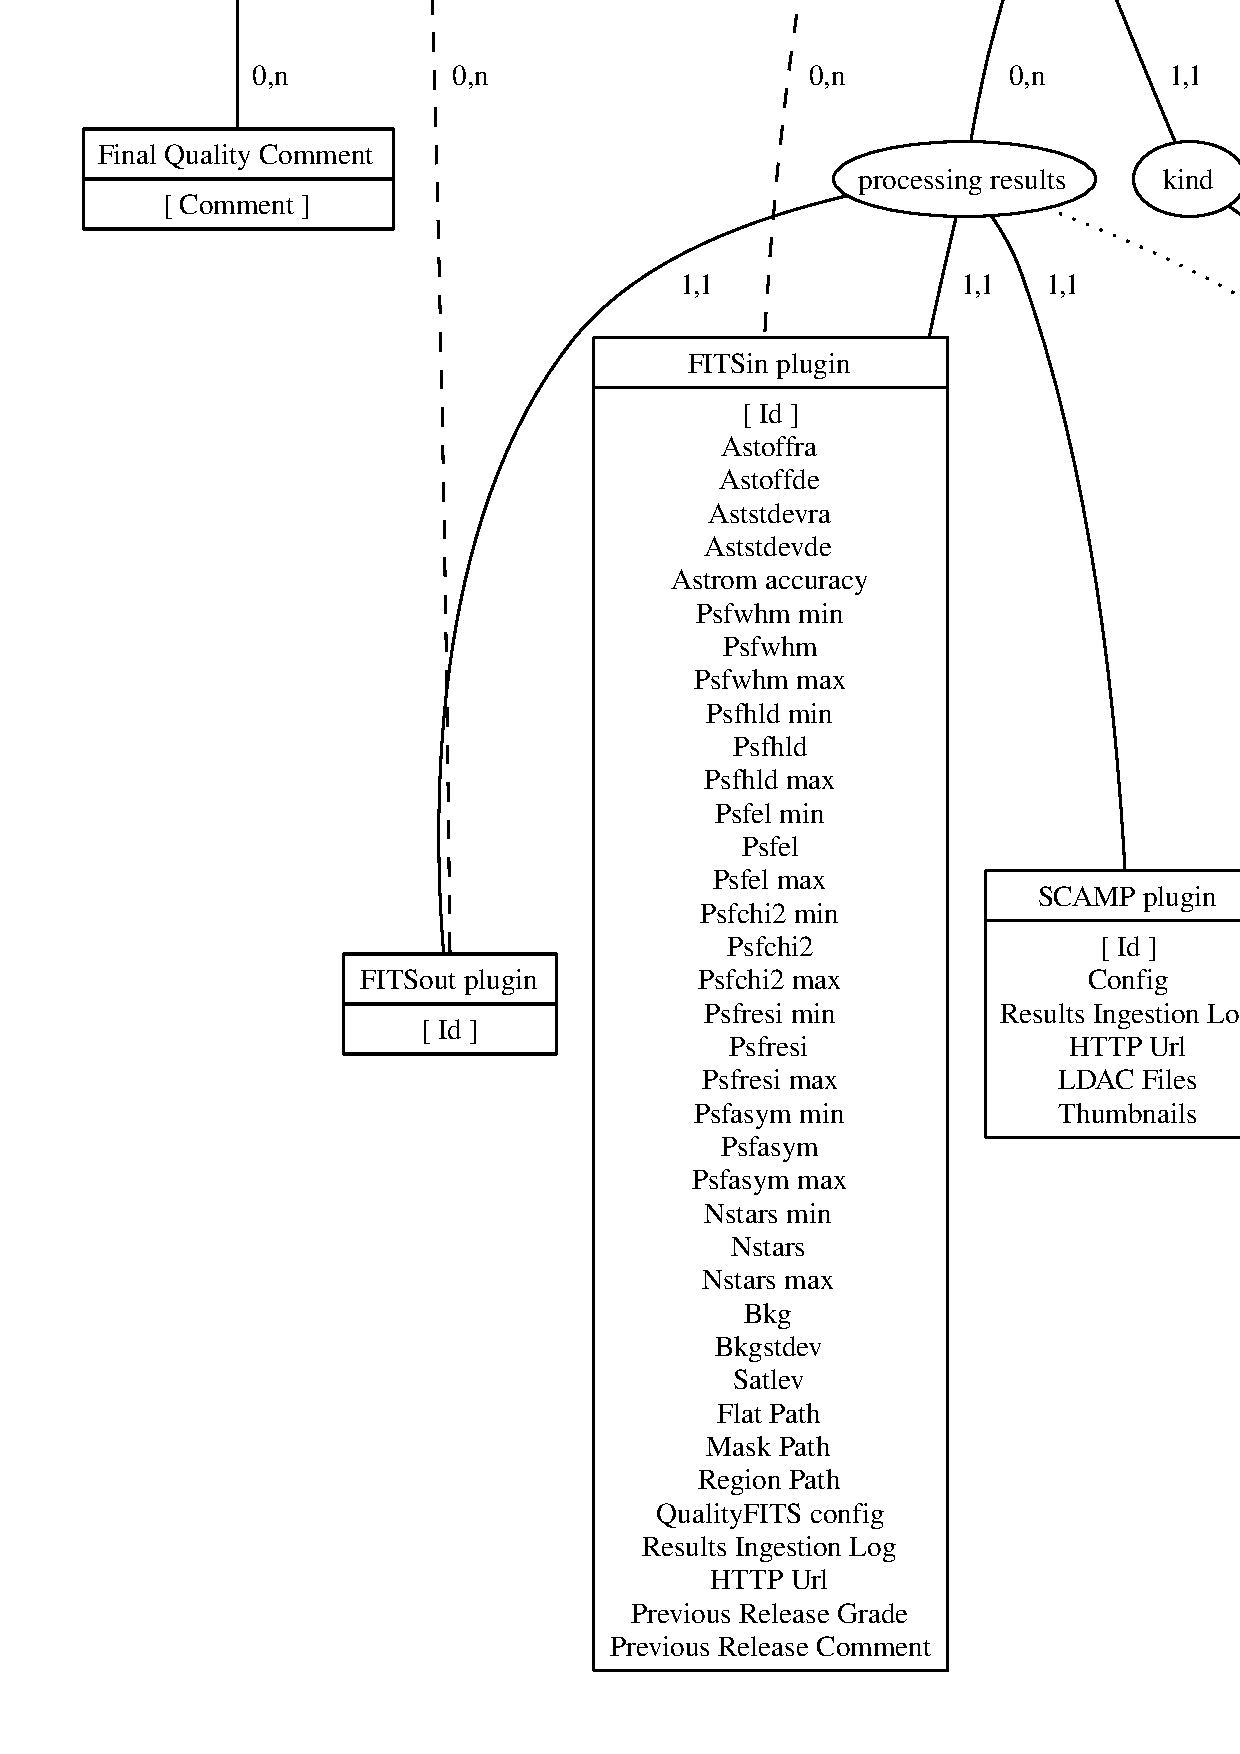
\includegraphics[totalheight=1.07\textheight]{mcd}
\caption[The Conceptual Model of Data]{The conceptual model of data (MCD). Properties surrounded with brackets are entities identifiers. The \emph{User}  entity (and its relations) is displayed with a dashed style because it is part of the standard Django's database model.}
\label{fig:mcd}
\end{figure}

\section{The \codasyl Logical Model}

\begin{figure}[p]
\centering
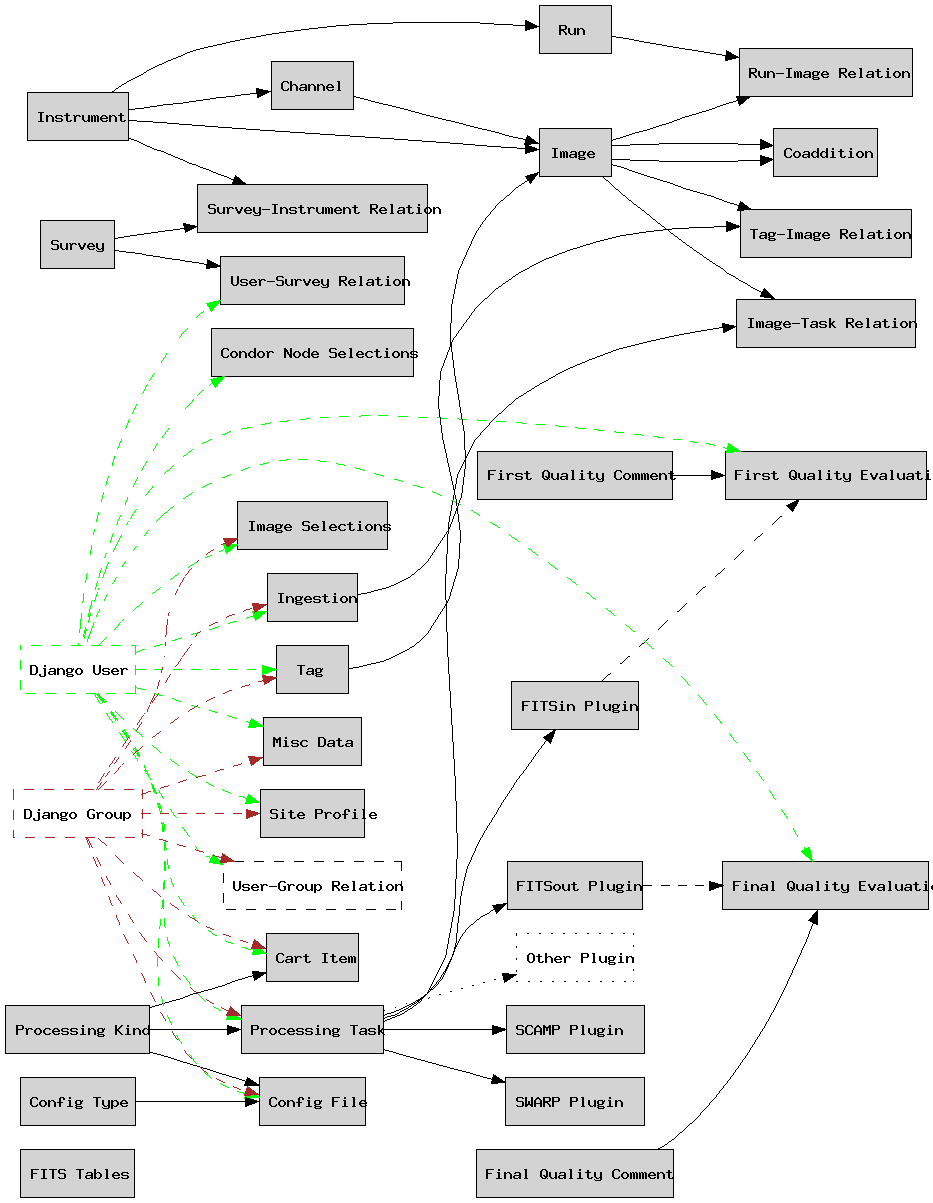
\includegraphics[width=\textwidth]{codasyl}
\caption[The \codasyl Logical Model]{The \codasyl logical model resulting of transformation rules applied to the previous {\sc MCD} model. The \emph{Django User} record is displayed with a dashed style because it is part of the standard Django's database model.}
\label{fig:codasyl}
\end{figure}

\section{The Relationnal Logical Model Of Data}
Here is the relationnal logical model of data used to design the database:

\begin{enumerate}
\sc
\item Astrophoto Calibration (\underline{Astrophoto Id}, Astrefcat, XML Path, Flat Field, Output ZP)
\item AstrophotoCalibration-Image Relation (\underline{Calibration Id, Astrophoto Id, Image Id})
\item Calibration Kit (\underline{Calibration Kit Id}, Name, Bad Pix Mask, Flat Field)
\item Cart Item (\underline{Item Id}, Django's User Id, Processing Kind Id, Name, Data, Date)
\item Channel (\underline{Channel Id}, Instrument Id, Name, Wave Length, Url, Wave Curve, Trans Curve, Mag Offsets)
\item Coaddition (\underline{Coaddition Id}, \ldots{})
\item Config File (\underline{Config Id}, Django's User Id, Processing Kind Id, Name, Content, Data, Date)
\item Final Quality Comment (\underline{Final Comment Id}, Comment)
\item Final Quality Evaluation (\underline{Django's User Id, FITSout Id}, Final Comment Id, Date, Grade, Custom Comment)
\item First Quality Comment (\underline{First Comment Id}, Comment)
\item First Quality Evaluation (\underline{Django's User Id, FITSin Id}, First Comment Id, Date, Grade, Custom Comment)
\item FITS Tables (\underline{Table Id}, Name, Instrument, Channel, Run, QSO Status, Object, FITS Table, Absorption, Absorption Err, Is Phot)
\item FITSIn Plugin (\underline{FITSIn Id}, Processing Task Id, RA offset, Dec offset, RA std dev, Dec std dev, Minimum PSF FWHM, Average PSF FWHM, Maximum PSF FWHM, Minimum PSF half-light diameter, Average PSF half-light diameter, Maximum PSF half-light diameter, Minimum PSF elongation, Average PSF elongation, Maximum PSF elongation, Minimum PSF chi2/d.o.f., Average PSF chi2/d.o.f., Maximum PSF chi2/d.o.f., Minimum PSF residuals, Average PSF residuals, Maximum PSF residuals, Minimum PSF asymmetry, Average PSF asymmetry, Maximum PSF asymmetry, Minimum number of PSF stars, Average number of PSF stars, Maximum number of PSF stars, Median background, Background RMS, Saturation level, Flat Path, Mask Path, Region Path, QualityFITS Config, Results Ingestion Log, HTTP Url, Previous Release Grade, Previous Release Comment)
\item FITSOut Plugin (\underline{FITSOut Id}, Processing Task Id)
\item Image (\underline{Image Id}, Calibration Kit Id, Ingestion Id, Channel Id, Instrument Id, Name, Sky Footprint, Path, Alpha, Delta, Equinox, Object, Date Obs, Exp time, Photc Header, Photc Custom, Photk, Airmass, Absorption, Checksum, Gain, Ingestion Date, Flat, Mask, Reg, QSO Status)
\item Image-Task Relation (\underline{I--T Id, Image Id, Processing Task Id}) 
\item Image Selections (\underline{Selection Id}, Django's User Id, Name, Data, Date)
\item Ingestion (\underline{Ingestion Id}, Django's User Id, Label, Start Ingestion Date, End Ingestion Date, Email, Path, Check Fitsverify, Check QSO Status, Check Multiple Ingestion, Exit Code, Report)
\item Instrument (\underline{Instrument Id}, Name, Telescope, Url, Timezone, Altitude, Nchips, Astrinstru\_key, Photinstru\_key, Path)
\item Misc Data (\underline{Misc Id}, Django's User Id, Key, Data, Date)
\item Processing Kind (\underline{Processing Kind Id}, Internal Name, Label)
\item Processing Task (\underline{Processing Task Id}, Django's User Id, Processing Kind Id, Start Date, End Date, Success, Error Log, Hostname, Results Output Directory, Title)
\item Run (\underline{Run Id}, Instrument Id, Name, PI, Url, Email, Process Request Date, Date Start, Date End, Date Download, Release Date)
\item Run-Image Relation (\underline{R--I Id, Image Id, Run Id}) 
\item SCAMP Plugin (\underline{SCAMP Id}, Processing Task Id, Config, Results Ingestion Log, HTTP Url, LDAC Files, Thumbnails)
\item Survey (\underline{Survey Id}, Name, Comment, Url)
\item Survey-Instrument Relation (\underline{S--I Id, Survey Id, Instrument Id}) 
\end{enumerate}

\begin{table}[!h]
\centering
\footnotesize{
\begin{tabular}{|l|l|l|l|l|}
\hline
CODASYL Record name & DB table name & Django's class(model) name\\
\hline
Astrophoto Calibration & {\tt youpi\_astrophotocalibration} & {\tt Astrophotocalibration}\\
AstrophotoCalibration-Image Relation & {\tt youpi\_rel\_ai} & {\tt Rel\_ai}\\
Calibration Kit & {\tt youpi\_calibrationkit} & {\tt CalibrationKit}\\
Cart Item & {\tt youpi\_cartitem} & {\tt CartItem}\\
Channel & {\tt youpi\_channel} & {\tt Channel}\\
Coaddition & {\tt youpi\_coaddition} & {\tt Coaddition}\\
Config File & {\tt youpi\_configfile} & {\tt ConfigFile}\\
Final Quality Comment & {\tt youpi\_finalqcomment} & {\tt FinalQComment}\\
Final Quality Evaluation & {\tt youpi\_finalqeval} & {\tt FinalQEval}\\
First Quality Comment & {\tt youpi\_firstqcomment} & {\tt FirstQComment}\\
First Quality Evaluation & {\tt youpi\_firstqeval} & {\tt FirstQEval}\\
FITS Tables & {\tt youpi\_fitstables} & {\tt Fitstables}\\
FITSIn Plugin & {\tt youpi\_plugin\_fitsin} & {\tt Plugin\_fitsin}\\
FITSOut Plugin & {\tt youpi\_plugin\_fitsout} & {\tt Plugin\_fitsout}\\
Image & {\tt youpi\_image} & {\tt Image}\\
Image-Task Relation & {\tt youpi\_rel\_it} & {\tt Rel\_it}\\
Image Selections & {\tt youpi\_imageselections} & {\tt ImageSelections}\\
Ingestion & {\tt youpi\_ingestion} & {\tt Ingestion}\\
Instrument & {\tt youpi\_instrument} & {\tt Instrument}\\
Misc Data & {\tt youpi\_miscdata} & {\tt MiscData}\\
Processing Kind & {\tt youpi\_processing\_kind} & {\tt Processing\_kind}\\
Processing Task & {\tt youpi\_processing\_task} & {\tt Processing\_task}\\
Run & {\tt youpi\_run} & {\tt Run}\\
Run-Image Relation & {\tt youpi\_rel\_ri} & {\tt Rel\_ri}\\
SCAMP Plugin & {\tt youpi\_plugin\_scamp} & {\tt Plugin\_scamp}\\
Survey & {\tt youpi\_survey} & {\tt Survey}\\
Survey-Instrument Relation & {\tt youpi\_rel\_si} & {\tt Rel\_si}\\
\hline
\end{tabular}}
\caption{Record--Table name mappings}
\end{table}


\end{document}
